% Created 2021-04-29 Thu 18:26
% Intended LaTeX compiler: pdflatex
\documentclass[11pt]{article}
\usepackage[utf8]{inputenc}
\usepackage[T1]{fontenc}
\usepackage{graphicx}
\usepackage{grffile}
\usepackage{longtable}
\usepackage{wrapfig}
\usepackage{rotating}
\usepackage[normalem]{ulem}
\usepackage{amsmath}
\usepackage{textcomp}
\usepackage{amssymb}
\usepackage{capt-of}
\usepackage{hyperref}
\usepackage[margin=0.5in]{geometry}
\usepackage{pgfplots}
\author{Hee Hwang and Sudarshan Raghavan}
\date{\today}
\title{Tasks}
\hypersetup{
 pdfauthor={Hee Hwang and Sudarshan Raghavan},
 pdftitle={Tasks},
 pdfkeywords={},
 pdfsubject={},
 pdfcreator={Emacs 26.3 (Org mode 9.1.9)}, 
 pdflang={English}}
\begin{document}

\maketitle






\section{Baseline}
\label{sec:org1e5a201}
ACL  : Citation Intent Classification\\
Hyper: HyperPartisan News Detection\\
RCT  : Randomized Controlled Trials

\subsection{Baseline}
\label{sec:orge3973ea}
\begin{center}
\begin{tabular}{|c|c|c|c|c|}
\hline
Task & train & dev & test & Classes\\
\hline
ACL & 1688 & 114 & 139 & 6\\
\hline
Hyper & 516 & 64 & 65 & 2\\
\hline
RCT-sample & 500 & 30212 & 30135 & 5\\
\hline
RCT-200k & 180040 & 30212 & 30135 & 5\\
\hline
\end{tabular}
\end{center}




\section{Tables \& Plots}
\label{sec:org732747b}

\subsection{Augmentation by Distance}
\label{sec:org9936a54}
\subsubsection{Size Table}
\label{sec:org72fbbe4}
\begin{center}
\begin{tabular}{|c|c|c|c|}
\hline
Max Distance & ACL & Hyper & RCT\\
\hline
Baseline & 1688 (100\%) & 516 (100\%) & 500(100\%)\\
\hline
24 & 1746 (103\%) & 551 (106\%) & 686(137\%)\\
\hline
26 & 1815 (107\%) & 567 (109\%) & 831(166\%)\\
\hline
28 & 1981 (117\%) & 606 (117\%) & 1065(213\%)\\
\hline
30 & 2253 (133\%) & 656 (127\%) & 1484(296\%)\\
\hline
32 & 2842 (168\%) & 742 (143\%) & 2105(421\%)\\
\hline
34 & 3848 (227\%) & 911 (176\%) & 2952(590\%)\\
\hline
36 & 5819 (344\%) & 1127 (218\%) & 4196(839\%)\\
\hline
\end{tabular}
\end{center}
\subsubsection{Size Plot}
\label{sec:org5135fa3}


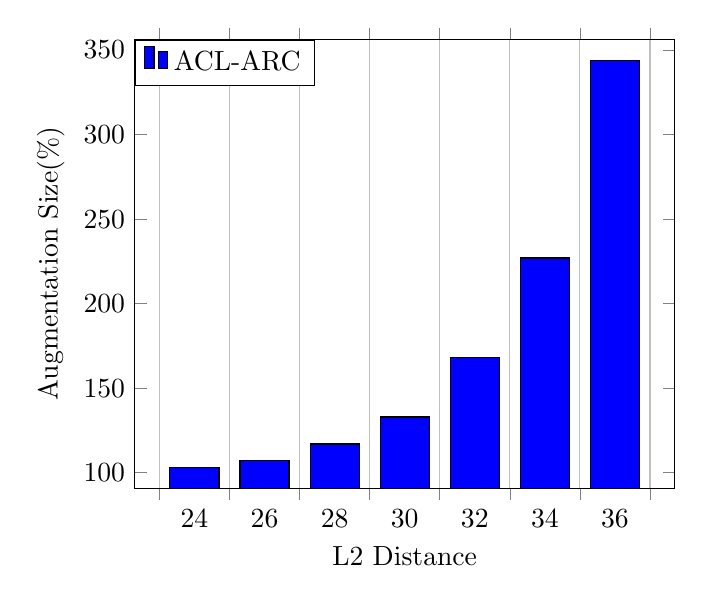
\begin{tikzpicture}
\begin{axis}[
	x tick label style={
		/pgf/number format/1000 sep=},
	xlabel=L2 Distance,
	ylabel=Augmentation Size(\%),
	enlargelimits=0.05,
	ybar interval=0.7,
  legend style={at={(0,1)},anchor=north west}
]
\addplot[fill=blue] 
	coordinates {(24,103) (26,107) (28,117) (30,133) (32,168) (34,227) (36,344) (38,344)};
\addlegendentry{ACL-ARC}
\end{axis}
\end{tikzpicture}

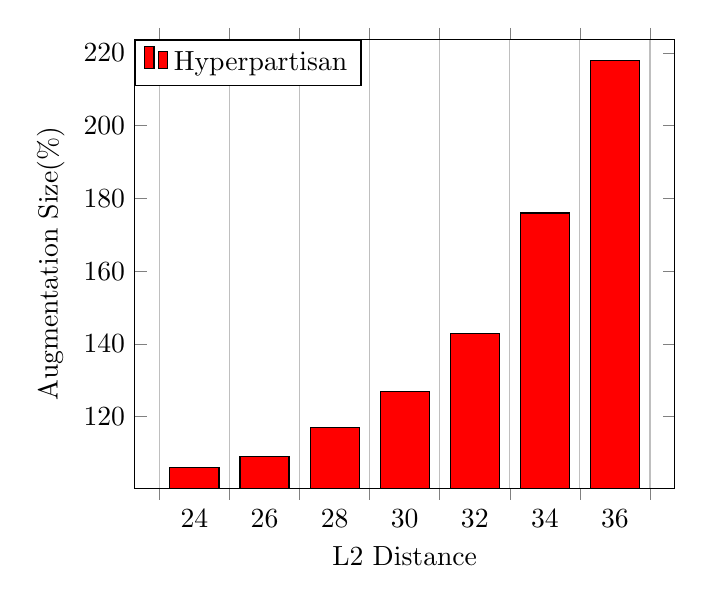
\begin{tikzpicture}
\begin{axis}[
	x tick label style={
		/pgf/number format/1000 sep=},
	xlabel=L2 Distance,
	ylabel=Augmentation Size(\%),
	enlargelimits=0.05,
	ybar interval=0.7,
  legend style={at={(0,1)},anchor=north west}
]
\addplot[fill=red]
	coordinates {(24,106) (26,109) (28,117) (30,127) (32,143) (34,176) (36,218) (38,218)};
\addlegendentry{Hyperpartisan}
\end{axis}
\end{tikzpicture}


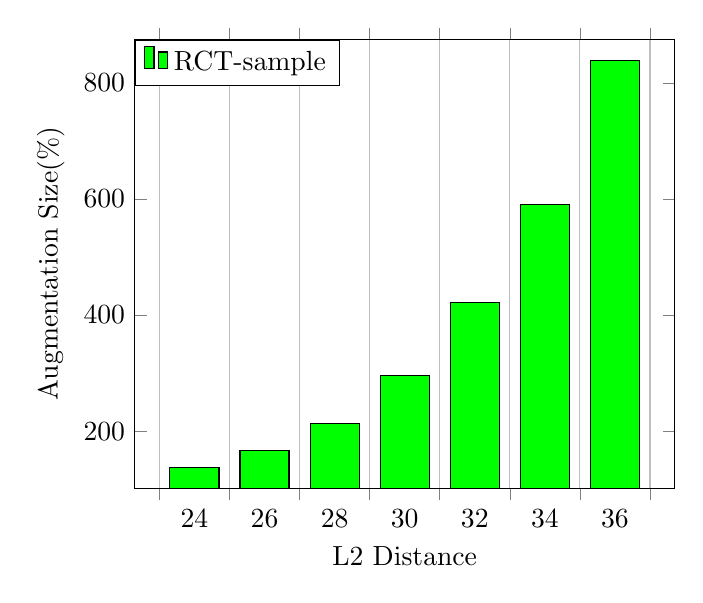
\begin{tikzpicture}
\begin{axis}[
	x tick label style={
		/pgf/number format/1000 sep=},
	xlabel=L2 Distance,
	ylabel=Augmentation Size(\%),
	enlargelimits=0.05,
	ybar interval=0.7,
  legend style={at={(0,1)},anchor=north west}
]
\addplot[fill=green]
	coordinates {(24,137) (26,166) (28,213) (30,296) (32,421) (34,590) (36,839) (38,839)};
\addlegendentry{RCT-sample}
\end{axis}
\end{tikzpicture}







\subsubsection{F1 Table}
\label{sec:org38dc177}
\begin{center}
\begin{tabular}{|c|c|c|c|}
\hline
Max Distance & ACL & Hyper & RCT\\
\hline
Baseline & 62.70 & 90.24 & \textbf{73.60}\\
\hline
24 & \textbf{73.45} & \textbf{93.66} & 70.06\\
\hline
26 & 71.71 & 81.98 & 69.19\\
\hline
28 & 66.17 & 92.03 & 64.50\\
\hline
30 & 65.34 & 81.32 & 60.57\\
\hline
32 & 61.64 & 88.85 & 58.77\\
\hline
34 & 59.56 & 83.75 & 53.47\\
\hline
36 & 59.22 & 88.70 & 53.27\\
\hline
\end{tabular}
\end{center}

\subsubsection{F1 Plot}
\label{sec:orge9a8ff9}
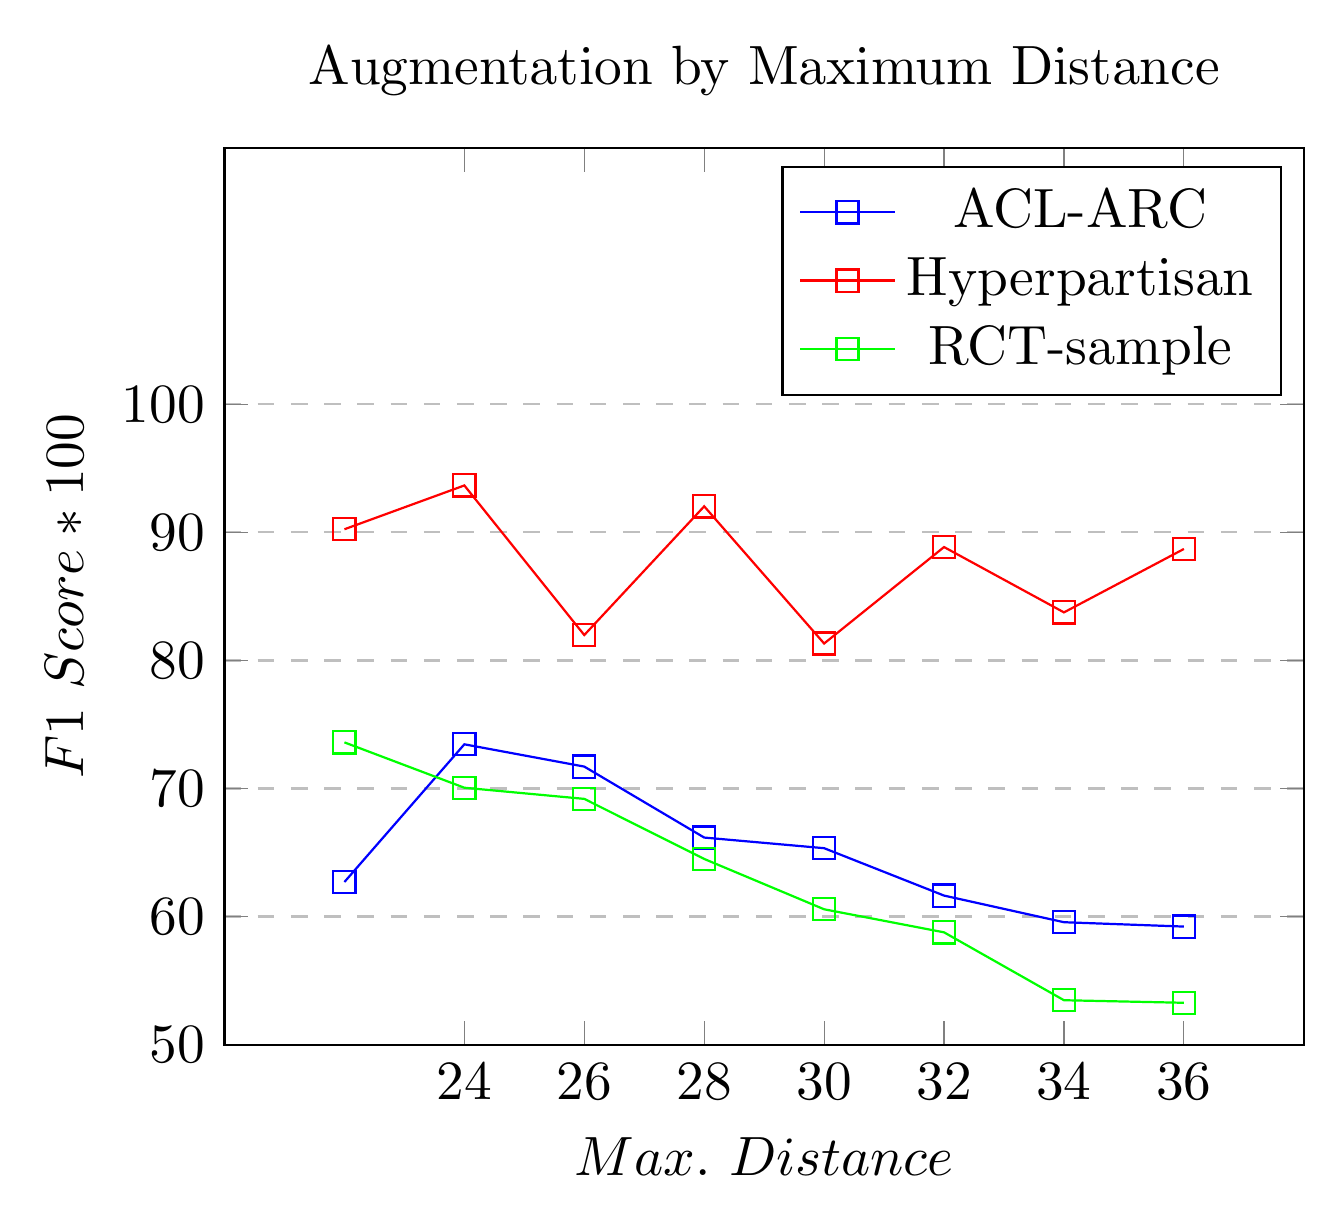
\begin{tikzpicture}[thick,scale=2.0]
\begin{axis}[
    title={Augmentation by Maximum Distance},
    xlabel={$Max.\ Distance$},
    ylabel={$F1\ Score * 100$},
    xmin=20, xmax=38,
           ymin=50, ymax=120,
    xtick={24,26,28,30,32,34,36},
    ytick={50,60,70,80,90,100},
    ymajorgrids=true,
    grid style=dashed,
]
\addplot[ 
    color=blue, 
    mark=square,
    ]
    coordinates {
    (22,62.70)(24,73.45)(26,71.71)(28,66.17)(30,65.34)(32,61.64)(34,59.56)(36,59.22)
    };
    \addlegendentry{ACL-ARC}

\addplot[
    color=red,
    mark=square,
    ]
    coordinates {
    (22,90.24)(24,93.66)(26,81.98)(28,92.03)(30,81.32)(32,88.85)(34,83.75)(36,88.70)
    };
    \addlegendentry{Hyperpartisan}

\addplot[
    color=green,
    mark=square,
    ]
    coordinates {
    (22,73.60)(24,70.06)(26,69.19)(28,64.50)(30,60.57)(32,58.77)(34,53.47)(36,53.27)
    };
    \addlegendentry{RCT-sample}

\end{axis}
\end{tikzpicture}


\subsection{Augmentation by Fixed Size}
\label{sec:org8623128}
\subsubsection{F1 Table}
\label{sec:org29a4e44}
\begin{center}
\begin{tabular}{|c|c|c|c|c|}
\hline
Dataset \# & ACL & Hyper & RCT & Interval\\
\hline
Baseline & 62.70 & 90.24 & \textbf{73.60} & -\\
\hline
1 & 66.24 & 90.38 & 73.26 & 0-3\%\\
\hline
2 & 62.01 & 84.16 & 70.29 & 3-6\%\\
\hline
3 & 60.48 & 86.99 & 71.89 & 6-9\%\\
\hline
4 & 61.68 & \textbf{98.40} & 72.59 & 9-12\%\\
\hline
5 & \textbf{69.66} & 95.22 & 71.69 & 12-15\%\\
\hline
6 & 65.31 & 95.22 & 72.51 & 15-18\%\\
\hline
7 & 65.00 & 93.50 & 71.66 & 18-21\%\\
\hline
8 & 66.22 & 77.82 & 71.99 & 21-24\%\\
\hline
9 & 58.84 & 91.93 & 70.14 & 24-27\%\\
\hline
10 & 57.61 & 86.78 & 70.44 & 27-30\%\\
\hline
\end{tabular}
\end{center}

\subsubsection{F1 Plot}
\label{sec:org363ce8e}
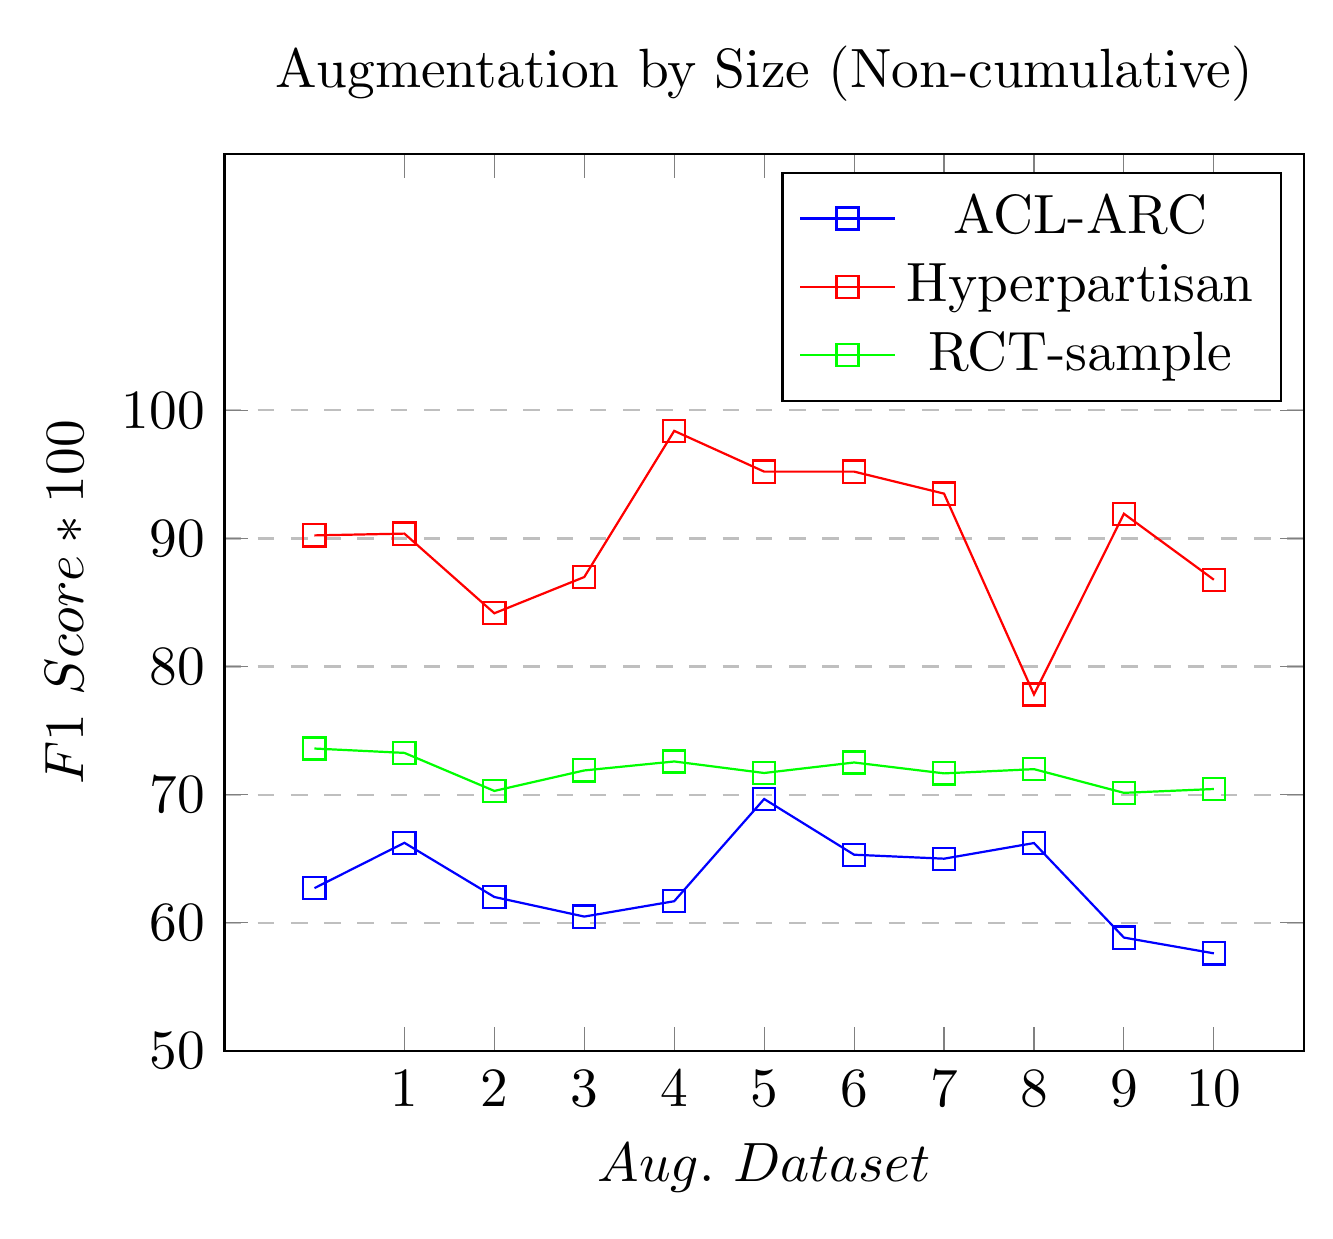
\begin{tikzpicture}[thick,scale=2.0]
\begin{axis}[
    title={Augmentation by Size (Non-cumulative)},
    xlabel={$Aug.\ Dataset$},
    ylabel={$F1\ Score * 100$},
    xmin=-1, xmax=11,
    ymin=50, ymax=120,
    xtick={1,2,3,4,5,6,7,8,9,10},
    ytick={50,60,70,80,90,100},
    ymajorgrids=true,
    grid style=dashed,
]

\addplot[ 
    color=blue, 
    mark=square, 
    ]
    coordinates {
    (0,62.70)(1,66.24)(2,62.01)(3,60.48)(4,61.68)(5,69.66)(6,65.31)(7,65.00)(8,66.22)(9,58.84)(10,57.61)
    };
    \addlegendentry{ACL-ARC}

 \addplot[
     color=red,
     mark=square,
     ]
     coordinates {
     (0,90.24)(1,90.38)(2,84.16)(3,86.99)(4,98.40)(5,95.22)(6,95.22)(7,93.50)(8,77.82)(9,91.93)(10,86.78)
     };
     \addlegendentry{Hyperpartisan}

 \addplot[
     color=green,
     mark=square,
     ]
     coordinates {
     (0,73.60)(1,73.26)(2,70.29)(3,71.89)(4,72.59)(5,71.69)(6,72.51)(7,71.66)(8,71.99)(9,70.14)(10,70.44)
     };
     \addlegendentry{RCT-sample}

\end{axis}
\end{tikzpicture}



\section{Baseline models:}
\label{sec:org043eda7}
\begin{itemize}
\item An off-the-shelf RoBERTa model that has been finetuned to perform classification for each of the downstream tasks
\end{itemize}

\section{Augmentation Model}
\label{sec:orge7956d4}
\begin{center}
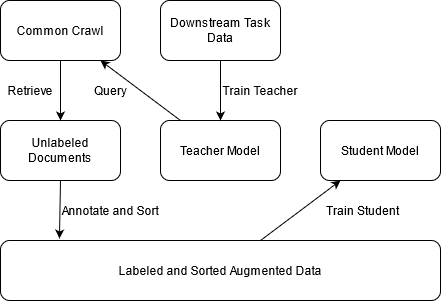
\includegraphics[width=.9\linewidth]{./png/da.png}
\end{center}


\section{Algorithm}
\label{sec:orgc8950b2}
\begin{verbatim}
1. Extract failed test examples from the baseline model
2. Retrieve passages/sentences from Common Crawl 
3. Apply augmentation strategy (i)-(iii)
4. Augment all the labelled CC data to the training data
5. Retrain RoBERTa on the augmented training set 
\end{verbatim}

\section{Augmentation Strategies}
\label{sec:org14cc945}
\begin{itemize}
\item Strategy (i)\\
Use baseline model (Teacher) to perform unsupervised labelling on retrieved CC data
\item Strategy (ii)\\
Using a task specific binary classifier, 
filter out retrieved CC data that is "out-domain"\\
Use baseline model (Teacher) to perform unsupervised labelling on the filtered "in-domain" CC data
\item Strategy (iii)\\
Using a task specific binary classifier, 
filter out retrieved CC data that is "out-domain"\\
Use ground truth labels of failed test examples and assign labels to the filtered "in-domain" CC data
\end{itemize}
\end{document}
